\chapter{A Private Cloud for MapReduce Applications}\label{cap:solucion}
\noindent This chapter introduces a novel solution combining the virtual infrastructure managed with OpenStack and the Hadoop implementation of MapReduce to conform a powerful computational tandem. \emph{qosh}, as this project has been called, will be described along this section moving from architecture to implementation.

\section{Architecture}\label{sec:diseno}
\noindent Figure \ref{fig:arquitecturaglobal} shows a high level portrait of qosh execution environment. The component that acts as interface between system and user is displayed on the right end. It abstracts the inherent difficulty in configuring the job execution context and in deploying the virtual cluster. Furthermore, qosh will keep track of submitted jobs, MapReduce \texttt{jar} files, input data and output results, with no need to walk the HDFS to search for data.

\begin{figure}[tbp]
\begin{center}
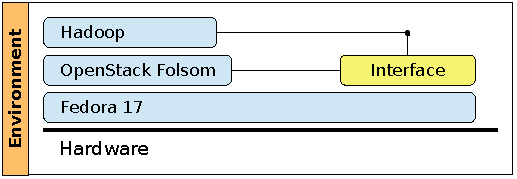
\includegraphics[width=0.65\textwidth]{imagenes/021.pdf}
 \caption{Global Architecture}
\label{fig:arquitecturaglobal}
\end{center}
\end{figure}

To streamline development, it is determined that the very first qosh version be tested on a personal computer. As shown on figure \ref{fig:arquitecturaglobal}, Fedora Linux is installed atop the hardware and OpenStack Folsom set up within. qosh will draw on the infrastructure provided by the local OpenStack configuration to deploy virtual Hadoop clusters. While it would be better to make qosh more flexible allowing for remote infrastructure consumption, it would also become harder to test.

Figure \ref{fig:arquitecturadetalle} shows a more detailed view on qosh design details. The VM contains a Hadoop installation ready to be put to use as soon as it was started. The VM life cycle is managed by OpenStack and its execution environment shaped by KVM, the chosen hypervisor. Besides, HDFS has been used as temporal persistence layer while the results are not send back to the controller --- the same machine in this testing environment. It shall be recalled that even though HDFS is a steady data store, the Hadoop VMs are created and removed for every work flow execution effectively destroying HDFS data at the end of processing each job. So, it is qosh's job to orchestrate data extraction before shutting down the virtual cluster.

\begin{figure}[tbp]
\begin{center}
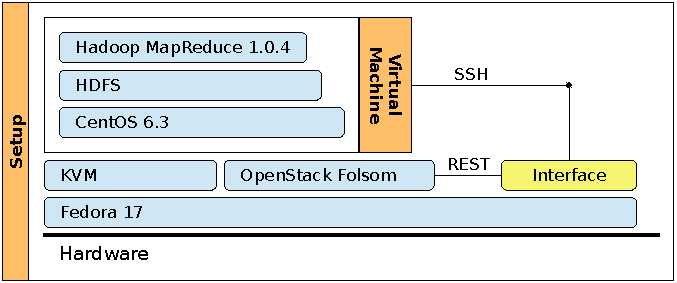
\includegraphics[width=0.85\textwidth]{imagenes/022.pdf}
 \caption{Detailed global architecture}
\label{fig:arquitecturadetalle}
\end{center}
\end{figure}

Figure \ref{fig:arquitecturainterfaz} shows the modular decomposition of qosh orchestration module.

\begin{figure}[bp]
\begin{center}
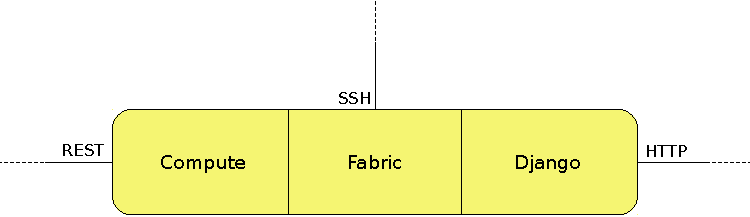
\includegraphics[width=0.8\textwidth]{imagenes/023.pdf}
 \caption{Core qosh modular decomposition}
\label{fig:arquitecturainterfaz}
\end{center}
\end{figure}

\begin{description}
 \item[Compute:] Acts as client to OpenStack REST API. It handles every interaction with the cloud decoupling qosh fromt the particular IaaS Cloud.
 \item[Django:] Is used in qosh to let users manage their MapReduce executions with ease via a web interface.
 \item[Fabric:] Is the Python library included in qosh to configure the virtual cluster deployment and destruction.
\end{description}

\subsection{Design Diagrams}\label{subsec:diagramasaltonivel}
\noindent Below are shown the design diagrams that make up the section on high level overview of the project.

\subsubsection{Django Components}\label{subsubsec:componentesdjango}
\noindent Figure \ref{fig:instalaciondjango} portrays modules adjacent to Django to support its operation.

\begin{figure}[bp]
\begin{center}
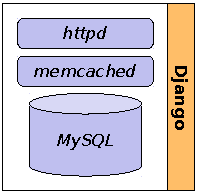
\includegraphics[width=0.23\textwidth]{imagenes/024.pdf}
 \caption{Django setup}
\label{fig:instalaciondjango}
\end{center}
\end{figure}

\begin{description}
 \item[Apache httpd:] Relied on to manage user interaction with OpenStack Dashboard, it may also be used to with qosh web interface. Initially, qosh depends on Python web server module to handle user requests, but \emph{httpd} might be easily configured.
 \item[memcached:] Is employed to cache web pages in order to speedup load times.
 \item[MySQL:] Chosen relational DBMS to store job meta-data.
\end{description}


\subsubsection{Use Cases Diagram}\label{subsubsec:casosuso}
\noindent Figure \ref{fig:casosuso} displays the set of use cases that have been considered for qosh. It reflects the five fundamental agents comprising the system.

\begin{figure}[tbp]
\begin{center}
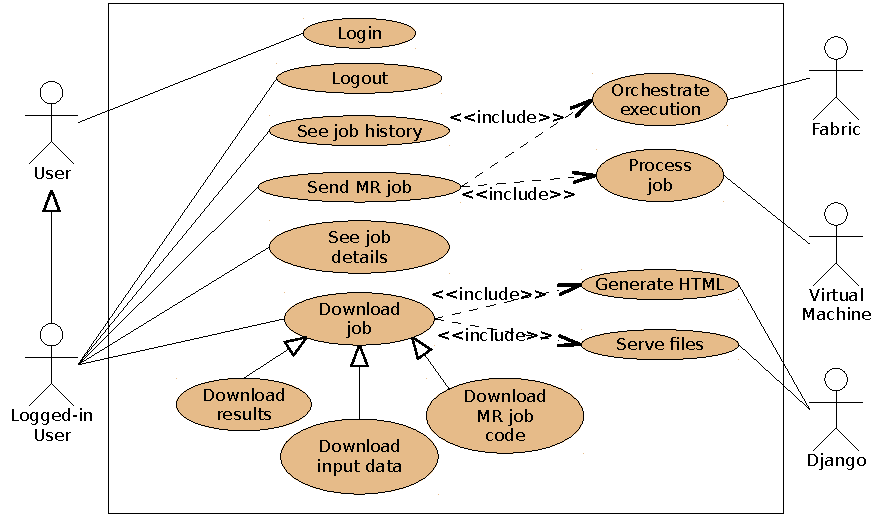
\includegraphics[width=0.99\textwidth]{imagenes/025.pdf}
 \caption{Use Cases Diagram}
\label{fig:casosuso}
\end{center}
\end{figure}

\subsubsection{Machine State Diagram}\label{subsubsec:navegacion}
\noindent Figure \ref{fig:navegacion} presents a summary on the navigation flow across the web interface. An example interaction is subsequently described.

Initially, the user is presented the \emph{Login} page so that he/she could log into qosh. If the supplied credentials were cleared --- the user must be previously registered in Keystone as user/pass is shared with qosh ---, the \emph{Main} page is shown. From there the user may \emph{Configure Job} or go over the \emph{Job History} to get some \emph{Job Details}.

\begin{figure}[tbp]
\begin{center}
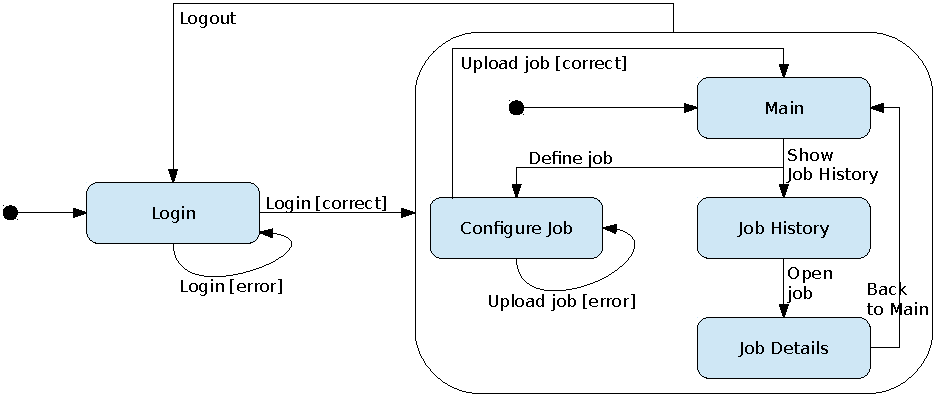
\includegraphics[width=0.99\textwidth]{imagenes/026.pdf}
 \caption{Web interface transitions}
\label{fig:navegacion}
\end{center}
\end{figure}

\subsubsection{Class Diagram --- Compute Module}\label{subsubsec:diagramaclasescompute}
\noindent Figure \ref{fig:diagramaclasescompute1} shows a small Class Diagram describing how the REST client is related to Fabric and Python.

\begin{description}
 \item[json:] Parses structured JSON-formated data and permits its manipulation. OpenStack REST API understands both XML and JSON.
 \item[Exception:] Python class representing a generic exception.
 \item[ServiceError:] Extends \texttt{Exception} to notify and handle any error that may be raised during execution. It's objects have two properties: an HTTP error code and error description.
 \item[Environment:] Contains the set of global options for configuring the virtual deployment.
 \item[httplib:] The Python module containing functions, classes and helpers toward interacting with HTTP connections. qosh banks on it to help consume the OpenStack REST service.
\end{description}

\begin{figure}[tbp]
\begin{center}
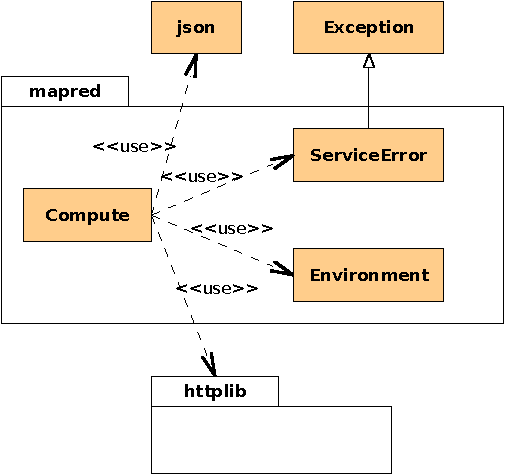
\includegraphics[width=0.5\textwidth]{imagenes/027.pdf}
 \caption{Class Diagram --- Compute module (I)}
\label{fig:diagramaclasescompute1}
\end{center}
\end{figure}

\section{Implementation}\label{sec:implementacion}
\noindent All the three modules conforming qosh core have been written in Python. The tests of the first version run over Fabric 1.4.3, Django 1.4.2 and Python 2.7.3. The configuration inside the VM is carried out by three \emph{Bash-Script}s in three different instants in the VM life cycle: before bringing the network up, after having completed the boot sequence and before shutdown. They will be detailed in section \ref{subsec:maquinavirtual}.

\subsection{Hadoop Virtual Machine}\label{subsec:maquinavirtual}
\noindent The Hadoop virtual machine is a vital asset for the qosh project; in the end it is Hadoop who executes work flows. The versions configured are Hadoop 1.0.4 and Oracle JRE 1.7. Installing and tunning every service in the VM has not been a complex process, whereas it has been long and interesting enough, for it is potentially reusable to create other customized VMs, to list every step followed to complete the setup.

\begin{itemize}
 \item In the local development machine the \emph{Virtual Machine Manager} (package \texttt{virt-manager}) was installed with \texttt{yum}. \texttt{yum} automatically installed dependent libraries like \texttt{libvirt}, the Kernel Virtual Machine hypervisor module (KVM) and a wrapper to handle it (\texttt{qemu-kvm}).
 \item Through the Virtual Machine Manager, a VM with 1 GB of RAM, 4 GB for the drive image within a \texttt{qcow2} container and both APIC and ACPI was created anew.
 \item A minimal network install of CentOS 6.3 was carried through. \emph{Basic Server} was chosen as initial package set on a single ext4 partition --- no swap partition --- without LVM.
 \item After the initial boot sequence, the distribution was put to the latest stable version available.
 \item The Oracle JRE 1.7 and Hadoop 1.0.4 were downloaded from official sources and subsequently installed on the VM.
 \item A new user (\emph{hduser}) was registered and set \emph{hadoop} as its primary group. As a result, the permission of the files related to Hadoop --- configuration files and scripts ---- were updated to allow this new user to launch and kill MapReduce jobs.
 \item \texttt{sshd} was tuned to disable superuser connections and user/pass authentication method; only ssh tunnels cleared by keypairs will be permitted.
 \item Three scripts --- similar to Ubuntu \texttt{cloud-init} scripts --- were written to \texttt{/etc/init.d/cloud-*} to customize part of the VM behavior. An important feature of them being they manage injecting the public part of the keypair used for authentication into the VM file system --- in \texttt{/home/hduser/.ssh/authorized\_keys} --- when it boots, so the owner of the private part can authenticate.
 \item The \texttt{yum groups} utility was applied to remove unused services like \emph{X-server}.
 \item From the local machine the VM was terminated and its drive image was mounted with \texttt{qemu-nbd} to remove logs and user history from the VM. Then, a 5 GB zeroed-file was created with \texttt{dd} inside the VM file system, failing, for there was not enough free space to accommodate 5 GB within a 4 GB image, while filling the remaining space up with zeros. Just after that, \texttt{qemu-img} was invoked to compress the image into a new file.
 \item Next, \texttt{fdisk} was used locally to observe the VM file system block size and initial block number of the Hadoop partition --- the only partition. By multiplying both values the partition offset was obtained, allowing for the extraction of the Hadoop partition using \texttt{qemu-nbd} offset-mounting capabilities and \texttt{dd} to dump, again, to a new file.
 \item Finally, both the \emph{initram} and the kernel image were copied out from the VM to the local file system.
\end{itemize}

\subsection{Low Level Diagramas}\label{subsec:diagramasimpl}
\noindent Next comes the diagram set that exposes those features closer to qosh implementation.

\subsubsection{Class Diagram --- Compute Module}\label{subsubsec:implementacioncompute}
\noindent Figure \ref{fig:diagramaclasescompute2} expands the \emph{Compute} module details on figure \ref{fig:diagramaclasescompute1}. Notice that types on function signatures have been borrowed from Python syntax on dictionaries and lists for brevity.

\begin{figure}[tbp]
\begin{center}
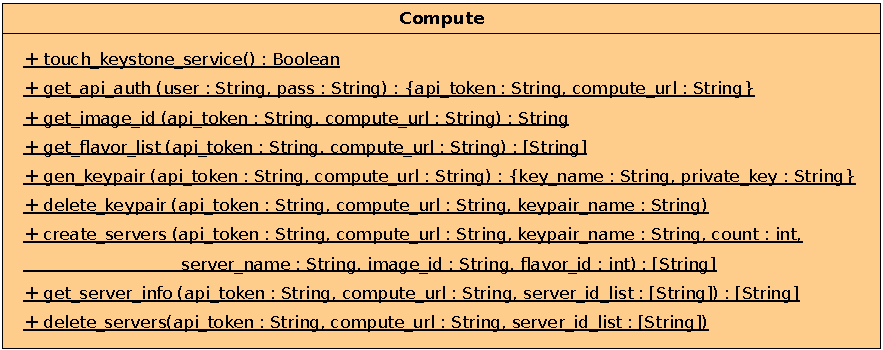
\includegraphics[width=0.99\textwidth]{imagenes/028.pdf}
 \caption{Class Diagram --- Compute module (II)}
\label{fig:diagramaclasescompute2}
\end{center}
\end{figure}

\begin{description}
 \item[List of type T:] \texttt{[T]}
 \item[Dictionary:] \texttt{\{<Key1> : <T1>, <Key2> : <T2> ... \}}
\end{description}

\subsubsection{Class Diagram --- Django and Fabric}\label{subsubsec:clasesdjangofabric}
\noindent Figure \ref{fig:djangoyfabric} exposes the relationship between the most important Django and Fabric modules.

\begin{figure}[tbp]
\begin{center}
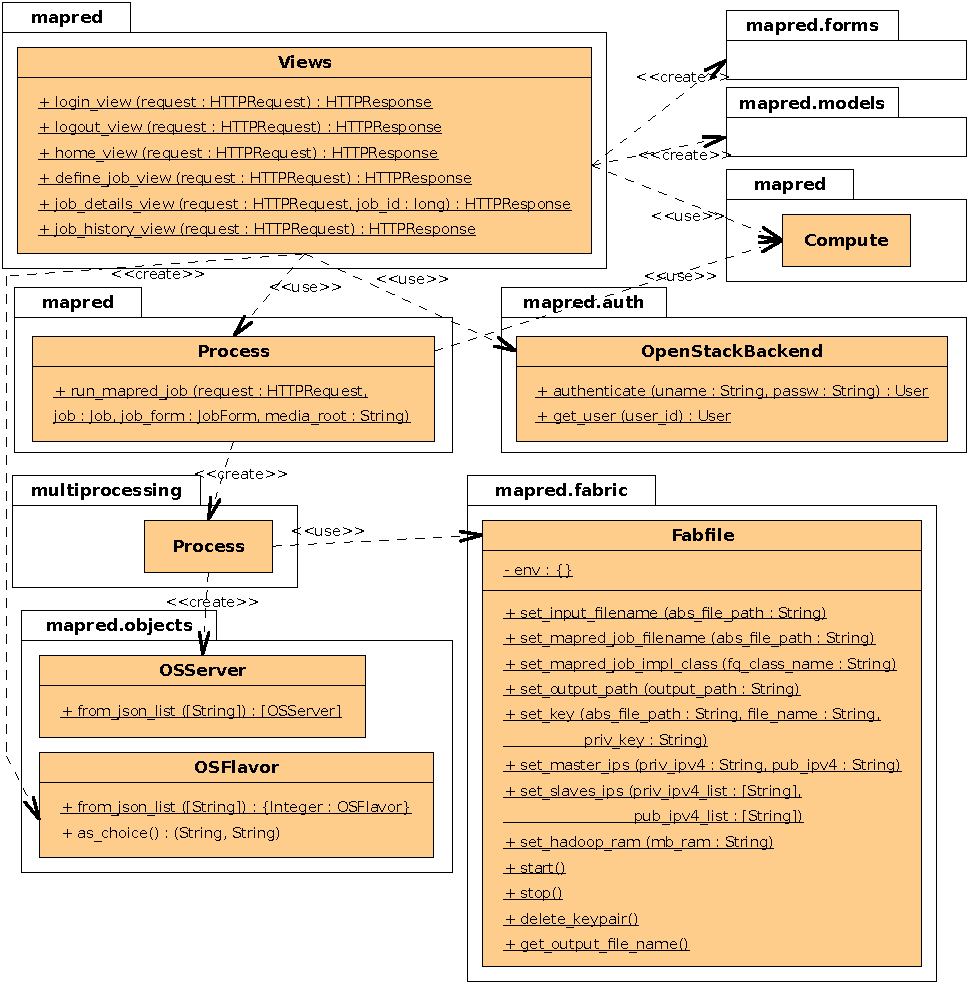
\includegraphics[width=0.99\textwidth]{imagenes/029.pdf}
 \caption{Class Diagram --- Django and Fabric}
\label{fig:djangoyfabric}
\end{center}
\end{figure}

\begin{description}
 \item[Views:] Is a delegate class implementing the behavior on each \emph{view}. It interacts with qosh Compute module to communicate with the cloud.
 \item[Process:] es una clase wrapper que encapsula tanto el comportamiento de creaci\'on de un proceso \texttt{multiprocessing.Process} como la funci\'on que ejecutar\'a el proceso creado. Esta funci\'on de \texttt{mapred.Process}, cuya firma no se ha incluido por simplicidad, controla el procesado de las instancias Hadoop a trav\'es de \texttt{Compute} y \texttt{Fabfile} (Fabric).
 \item[OpenStackBackend:] es un peque\~no backend que gestiona la conexi\'on de los usuarios. Django incluye un sistema bastante completo para manejar las credenciales de conexi\'on, pero en este proyecto hemos decidido apoyarnos en el de OpenStack para evitar la duplicidad de los usuarios, sus contrase\~nas y datos del perfil. Por tanto, el papel de este backend es hacer de \emph{puente} entre el sistema integrado de credenciales de Django y el de OpenStack; cada petici\'on de conexi\'on se reenv\'ia al \emph{pipe} de acceso a OpenStack. Es decir, s\'olo es necesario que el usuario est\'e registrado en el cloud soporte, OpenStack en nuestro caso, para lanzar trabajos MapReduce.
 \item[OSServer y OSFlavor:] son clases \emph{helper} que desacoplan a la interfaz del servicio REST. Crean representaciones equivalentes en forma de objetos de los JSON que procesan como resultado de las invocaciones de \texttt{Compute}.
\end{description}



\subsubsection{Diagrama de Clases --- Objetos de Django}\label{subsubsec:clasesobjetosdjango}
\noindent La figura \ref{fig:clasesobjetosdjango} contiene, en detalle, las relaciones entre las \emph{clases de objetos del modelo concreto} de Django.


\begin{figure}[tbp]
\begin{center}
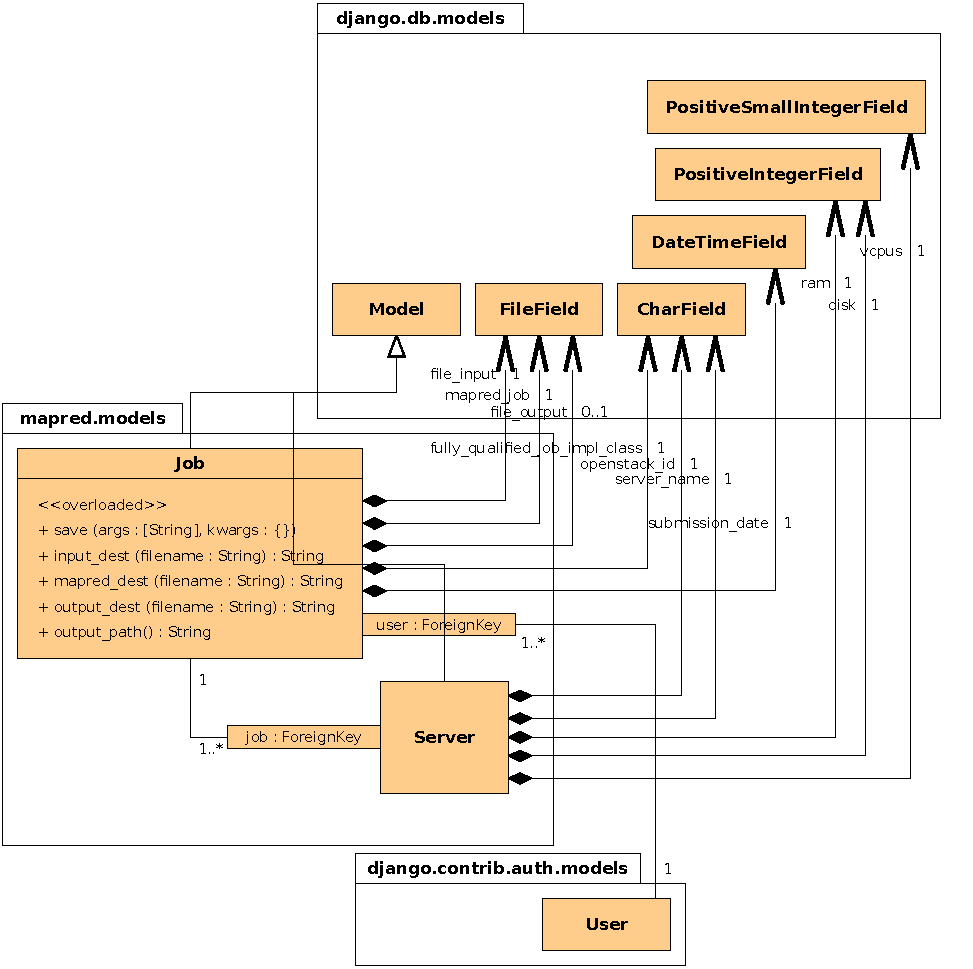
\includegraphics[width=0.99\textwidth]{imagenes/030.pdf}
 \caption{Diagrama de Clases --- Objetos de Django}
\label{fig:clasesobjetosdjango}
\end{center}
\end{figure}


\begin{description}
 \item[django.db.models:] este paquete lo proporciona la distribuci\'on de Django. Sirve de apoyo para escribir objetos del modelo de aplicaci\'on, basados en composiciones y extensiones de las clases contenidas.
  \begin{description}
   \item[Model:] es la clase base de los objetos del modelo, esto es, todo objeto de nuestro minimundo ha de ser \emph{descendiente} suyo. Usando esta clase y las definiciones de las clases de objetos, Django se encargar\'a de gestionar todo lo relativo a la persistencia de los objetos del modelo en una base de datos.
   \item[Fields:] son algunas de las implementaciones m\'as usuales de campos de inter\'es para los objetos que, junto con \texttt{Model}, permiten que Django establezca la morfolog\'ia del esquema l\'ogico de la base de datos asociada.
  \end{description}
 \item[Job:] representa un trabajo MapReduce para Hadoop. Comentar que se ha especializado la definici\'on del m\'etodo \texttt{save}, para poder organizar los trabajos en el sistema de ficheros por su identificador en la base de datos. Tal y como se ha comentado, la salvaguarda de informaci\'on de cada \texttt{Job} en una base datos corre a cargo de Django.
 \item[Server:] es la representaci\'on de la configuraci\'on individual de cada m\'aquina virtual que participe en un trabajo Hadoop MapReduce.
 \item[User:] es la clase interna de Django que almacena la informaci\'on de los usuarios de la interfaz. Se utiliza como \emph{Transfer Object} desde el sistema de autorizaci\'on de OpenStack como portador de los datos de los usuarios en cada \emph{sesi\'on}.
\end{description}


\subsubsection{Diagrama de Clases --- Formularios de Django}\label{subsubsec:clasesformulariosdjango}
\noindent La figura \ref{fig:clasesformulariosdjango} muestra la descomposici\'on en clases de los formularios que recogen las credenciales de acceso y la configuraci\'on del procesado. El paquete \texttt{django.forms} tiene organizaci\'on y finalidad id\'enticos al paquete \texttt{django.db.\\models} comentado anteriormente. En este caso \texttt{Form}, junto con los \texttt{Field} necesarios, es la clase extensible que aporta Django para concretar los formularios de usuario.

\begin{figure}[tbp]
\begin{center}
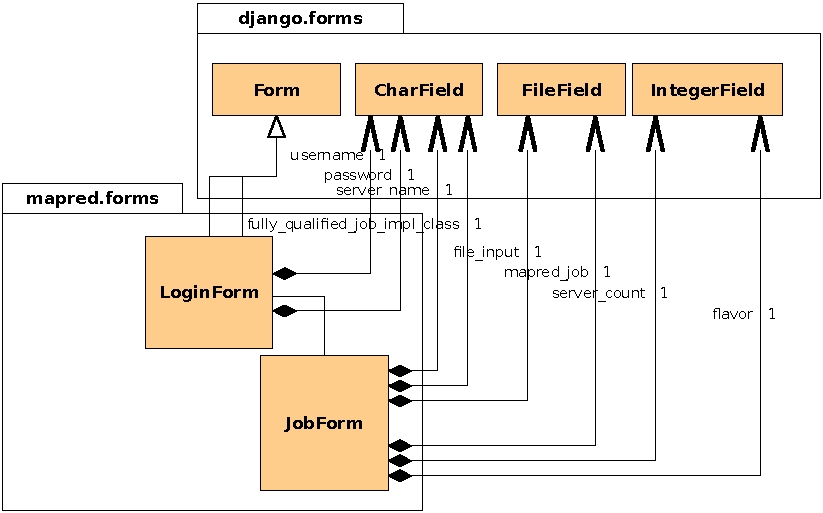
\includegraphics[width=0.99\textwidth]{imagenes/031.pdf}
 \caption{Diagrama de Clases --- Formularios de Django}
\label{fig:clasesformulariosdjango}
\end{center}
\end{figure}

\begin{description}
 \item[LoginForm:] formulario de conexi\'on de usuarios. Formado por un par de campos car\'acter que recogen el nombre de usuario y su contrase\~na en OpenStack.
 \item[JobForm:] es el formulario que permite definir la computaci\'on para \\MapReduce. Incluye: el prefijo del nombre de los servidores virtuales que se crear\'an, el nombre cualificado de la clase implementaci\'on de las funciones Map y Reduce, el fichero de entrada (paquete comprimido), el paquete \emph{Jar} que contiene la clase implementaci\'on, el n\'umero de servidores virtuales necesarios y su \emph{flavor} computacional.
\end{description}


\subsubsection{Diagrama Entidad-Relaci\'on}\label{subsubsec:entidadrelacion}
\noindent Se hab\'ia apuntado brevemente que Django posee la habilidad de construir autom\'aticamente el esquema l\'ogico de una base de datos relacional derivando el modelo de objetos escrito por el desarrollador. Era de esperar que la gesti\'on de las operaciones \emph{CRUD} (\emph{Create, Read, Update, Delete}) sobre las tuplas almacenadas tambi\'en estuviese implementada. La figura \ref{fig:entidadrelacion} muestra el diagrama Entidad-Relaci\'on correspondiente a la gesti\'on de trabajos. Se han omitido las entidades y relaciones adyacentes que gestionan las sesiones o las autorizaciones de los usuarios, entre otras, por transparencia.

\begin{figure}[tbp]
\begin{center}
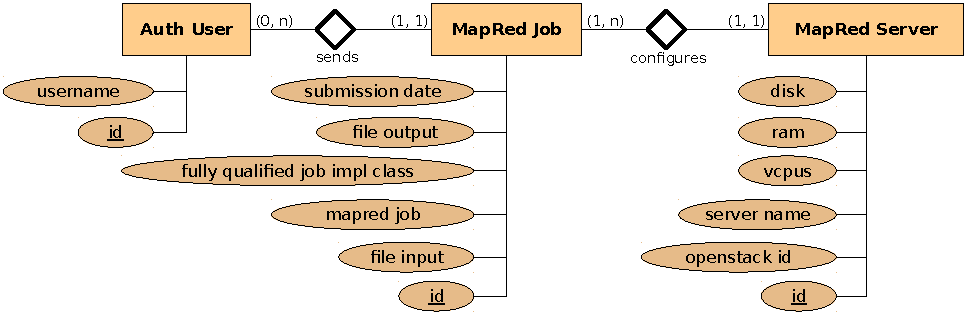
\includegraphics[width=0.99\textwidth]{imagenes/032.pdf}
 \caption{Diagrama Entidad-Relaci\'on}
\label{fig:entidadrelacion}
\end{center}
\end{figure}


\subsubsection{Diagrama de Secuencia}\label{subsubsec:secuencia}

\noindent Se presentan en las figuras \ref{fig:secuencia1} y \ref{fig:secuencia2} dos Diagramas de Secuencia. Reflejan el subconjunto m\'as interesante de los mensajes intercambiados entre las entidades participantes en un procesado MapReduce. Estamos suponiendo que no se produce ning\'un error, que el usuario est\'a conectado a la interfaz con sus credenciales, que introduce correctamente todos los datos de definici\'on del procesado y que posee la autorizaci\'on necesaria para lanzar m\'aquinas virtuales en OpenStack. La figura \ref{fig:secuencia1} contiene la interacci\'on completa. La \ref{fig:secuencia2} expone con detalle la activaci\'on posterior al mensaje \texttt{\#24} de la figura \ref{fig:secuencia1}.

\begin{figure}[tbp]
\begin{center}
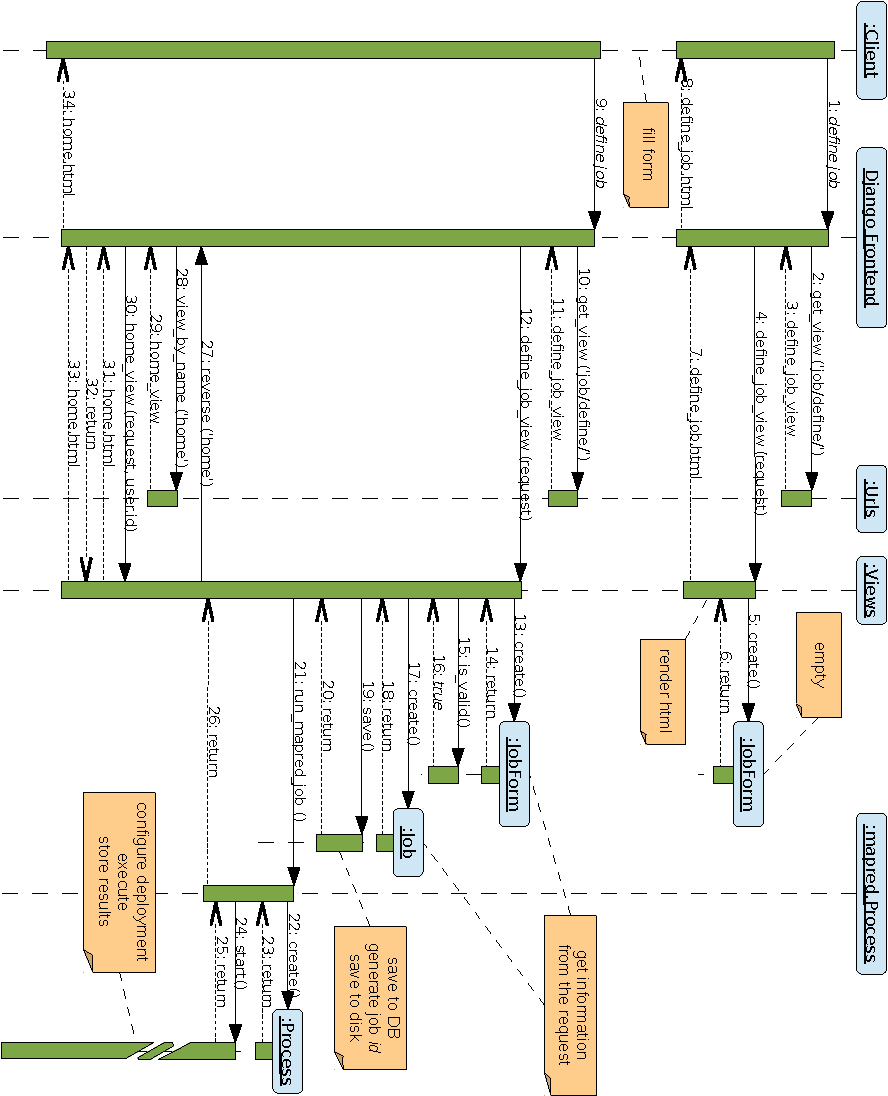
\includegraphics[width=0.99\textwidth]{imagenes/033.pdf}
 \caption{Diagrama de Secuencia (I)}
\label{fig:secuencia1}
\end{center}
\end{figure}

\begin{figure}[tbp]
\begin{center}
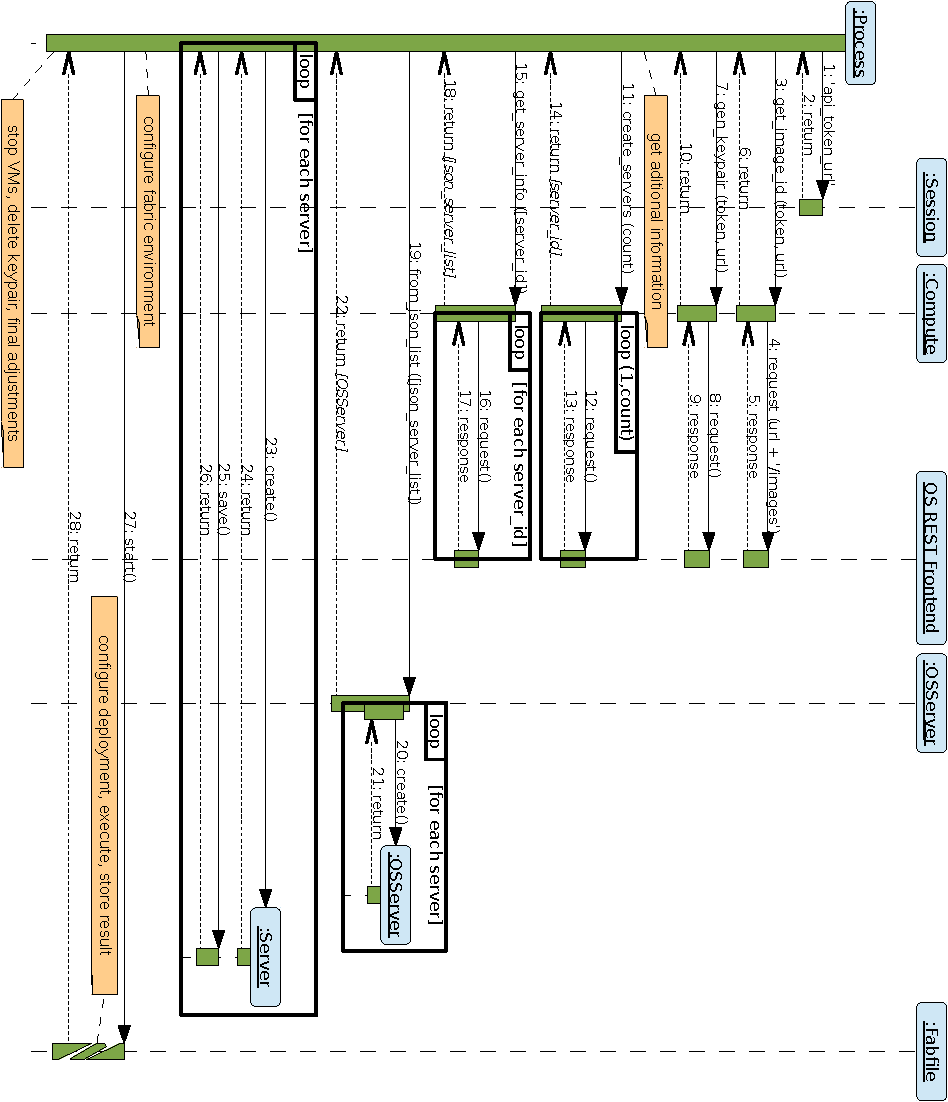
\includegraphics[width=0.99\textwidth]{imagenes/034.pdf}
 \caption{Diagrama de Secuencia (II)}
\label{fig:secuencia2}
\end{center}
\end{figure}

